%=====================================================================
\section{Thailand}\label{sec:thailand}

\subsection{Institutional setting}
Thailand's financial system combines a concentrated commercial banking sector, in which a small number of domestic systemically important banks (D-SIBs) account for most deposits and payments, with state-owned specialised financial institutions (SFIs) that serve retail, rural, housing and SME segments. A large non-bank payment and e-money sector operates under the Payment Systems Act B.E.~2560 (2017) \citep{thailand2017payment}. Virtual banks were licensed in 2025 under a framework issued in 2024 \citep{bot2024virtual}, and digital-asset exchanges and custodians are supervised by the securities regulator. The core payment infrastructure comprises the BOT-operated RTGS system (BAHTNET), the retail real-time payment system (PromptPay and related services operated by National ITMX) and card switching. The Cybersecurity Act B.E.~2562 (2019) designates the banking and financial sector as critical information infrastructure \citep{thailand2019cyber}, and the Thai Bankers' Association operates a sector CERT (TB-CERT).

The four Thai cases in our incident set---ATM malware at a state-owned bank (2016), web-application data leaks at two large banks (2018), a card-not-present fraud wave (2021) and remote-access malware on customers' phones (2022--2023)---involved no zero-day. Thai institutions nevertheless run the same commercial perimeter, MFT, mail, IT-management and virtualisation products that appear in the KEV catalogue, so they sit in the path of the same global mass-exploitation waves.

\subsection{Targets and vulnerable groups}
Table~\ref{tab:thai} and Figure~\ref{fig:thai} report the group framework. Groups with the highest \emph{target} index are the D-SIBs, payment FMIs, shared IT and cloud providers, the BOT's corporate and supervisory IT, and SFIs. Groups with the highest \emph{vulnerability} index are retail customers and their devices, payment and e-money providers, virtual banks, shared providers, digital-asset firms and non-bank lenders. Combining the two, three groups rank highest: shared IT and cloud providers ($R=0.72$; in the top three in 86\% of robustness draws), D-SIBs (0.67; 73\%) and SFIs (0.59; 52\%). Digital-asset exchanges and custodians (0.56) and non-bank payment providers (0.52) follow.

\begin{table}[!htbp]
\centering
\caption{Thai group framework: scores ($A$ attractiveness, $S$ systemic importance, $E$ exposure, $K$ concentration, $D$ defensive capacity), risk $R$, rank, 90\% rank interval and probability of ranking in the top three across 10,000 robustness draws. Scores are structured author judgements about groups, not assessments of institutions.}
\label{tab:thai}
\scriptsize
\resizebox{\textwidth}{!}{\begin{tabular}{p{0.30\textwidth}rrrrrrrrr}
\toprule
Group & $A$ & $S$ & $E$ & $K$ & $D$ & $R$ & Rank & 90\% rank & P(top 3) \\
\midrule
Shared IT and cloud service providers to the sector & 4 & 5 & 4 & 5 & 3 & 0.72 & 1 & 1--5 & 86 \\
Large systemically important banks & 5 & 5 & 5 & 4 & 5 & 0.67 & 2 & 1--6 & 73 \\
Specialised financial institutions (state-owned) & 4 & 4 & 4 & 4 & 3 & 0.59 & 3 & 1--8 & 52 \\
Digital-asset exchanges and custodians & 5 & 2 & 5 & 4 & 3 & 0.56 & 4 & 1--10 & 32 \\
Non-bank payment and e-money providers & 3 & 3 & 5 & 4 & 2 & 0.52 & 5 & 2--10 & 25 \\
Retail customers and their mobile devices & 3 & 2 & 5 & 4 & 1 & 0.47 & 6 & 2--11 & 11 \\
Other domestic commercial banks & 3 & 3 & 4 & 4 & 3 & 0.44 & 7 & 3--11 & 8 \\
Virtual banks (licensed 2025) & 3 & 2 & 5 & 5 & 3 & 0.43 & 8 & 4--11 & 5 \\
Bank of Thailand corporate and supervisory IT & 4 & 4 & 3 & 3 & 4 & 0.43 & 9 & 3--11 & 5 \\
Payment FMIs (RTGS; retail switch; card switch) & 5 & 5 & 2 & 3 & 5 & 0.40 & 10 & 4--11 & 2 \\
Non-bank lenders and card companies & 2 & 2 & 4 & 4 & 2 & 0.32 & 11 & 6--12 & 0 \\
Foreign bank branches and subsidiaries & 3 & 2 & 3 & 3 & 4 & 0.27 & 12 & 9--12 & 0 \\
\bottomrule
\end{tabular}}
\end{table}

\begin{figure}[!htbp]
\centering
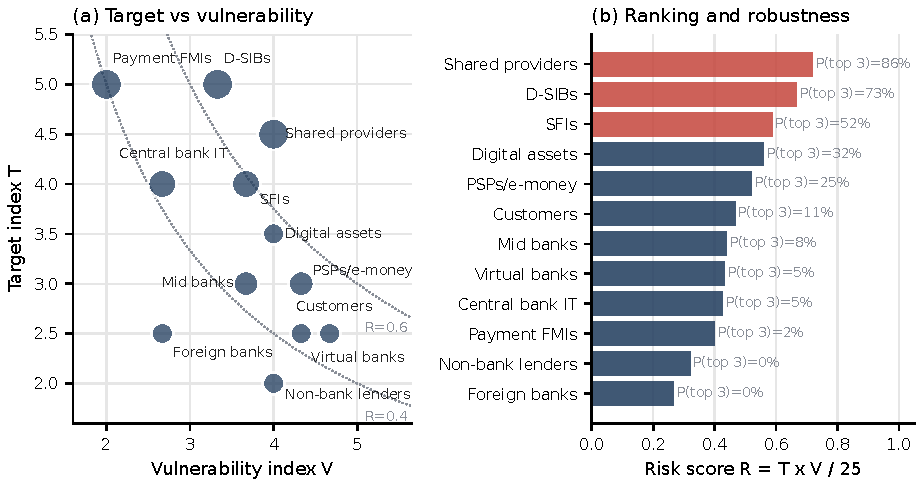
\includegraphics[width=\textwidth]{fig10_thai_groups.pdf}
\caption{Thai group framework. (a) Target index vs.\ vulnerability index; bubble size is systemic importance; dotted lines are iso-risk contours. (b) Risk score with the probability of ranking in the top three across robustness draws.}
\label{fig:thai}
\end{figure}

Three findings are robust to the perturbations. \emph{Shared providers rank at or near the top} because they combine one-to-many access with concentration: a single compromised outsourcer, cloud tenant or core-banking vendor creates correlated exposure across several banks, as the SolarWinds, MOVEit (via service providers) and CrowdStrike cases illustrate. \emph{D-SIBs are the main target but not the most vulnerable}: their defensive capacity offsets their exposure, yet their size makes any successful intrusion systemically relevant. \emph{Payment FMIs are high-value but low-vulnerability}: limited internet exposure and strong controls place them tenth, which is consistent with the absence of documented intrusions into core RTGS platforms in our incident set.

\paragraph{Answer to RQ5.} The likely \emph{targets} in Thailand are the D-SIBs, payment infrastructure, digital-asset platforms and the BOT itself. The groups most at \emph{risk} are shared IT providers, D-SIBs and SFIs. The most \emph{vulnerable} entry points are smaller non-bank payment firms, new virtual banks with concentrated cloud dependence, and customers' devices---the last mainly as a fraud channel that seldom needs zero-days. Whether Thai banks ``survive'' depends less on whether a Thailand-specific zero-day exists than on how quickly Thai institutions close exposure to global ones, and on whether a compromise at one shared provider can be contained.

%=====================================================================
\section{Scenario simulation}\label{sec:sim}

Tables~\ref{tab:simgroups}--\ref{tab:simparams} give the model's structure, calibration and scenarios. The base event rate of 86.7 exploited-vulnerability events per year across six enterprise layers comes from KEV. Edge and VPN products carry the highest rate (28.3 per year) and, with MFT, the highest zero-day share (0.61 and 0.67). For n-days, the median empirical KEV lag in these layers is 64 days. Scenario S0 represents conditions before 2022 (fewer zero-days, a 32-day time-to-exploit). S1 represents current conditions. S2 triples zero-day discovery and attacker throughput and shortens time-to-exploit to one day. S3 adds AI-enabled defence: patch times cut by 65\%, attack success reduced by 40\% through detection, and 30\% of bugs pre-empted. S4 adds vendor concentration to S2. S5 combines S3 with diversified vendor shares.

\begin{table}[!htbp]
\centering
\caption{Simulated institution groups (stylised; patch medians refer to critical internet-facing vulnerabilities).}
\label{tab:simgroups}
\small
\begin{tabular}{lrrrrrr}
\toprule
Group & Nodes & Payment share & Patch median (d) & Success $s_g$ & P(disrupt) & Attractiveness \\
\midrule
D-SIBs & 6 & 0.66 & 4 & 0.35 & 0.15 & 5 \\
Mid banks & 8 & 0.10 & 10 & 0.60 & 0.25 & 3 \\
Foreign banks & 12 & 0.06 & 7 & 0.45 & 0.20 & 3 \\
SFIs & 6 & 0.10 & 14 & 0.60 & 0.30 & 4 \\
Virtual banks & 3 & 0.01 & 5 & 0.60 & 0.30 & 3 \\
PSPs/e-money & 25 & 0.05 & 21 & 0.80 & 0.35 & 3 \\
Shared providers & 5 & 0.00 & 10 & 0.60 & 0.00 & 4 \\
Payment FMIs & 2 & 0.00 & 5 & 0.25 & 0.10 & 5 \\
\bottomrule
\end{tabular}
\end{table}

\begin{table}[!htbp]
\centering
\caption{Layer calibration from the KEV panel (CVEs published 2023--2025).}
\label{tab:simlayers}
\small
\resizebox{\textwidth}{!}{\begin{tabular}{lrrrrrr}
\toprule
Layer & Edge/VPN & MFT & Email/collab & IT mgmt/RMM & Virtualisation & Enterprise apps \\
\midrule
Event rate per year (KEV-calibrated) & 28.3 & 5 & 12.7 & 14.3 & 6.3 & 20 \\
Share exploited as zero-day & 0.61 & 0.67 & 0.26 & 0.37 & 0.26 & 0.18 \\
\bottomrule
\end{tabular}}
\end{table}

\begin{table}[!htbp]
\centering
\caption{Scenario parameters. $m_d$: discovery multiplier; $\tau$: zero-day copycat time-to-exploit (days); $\kappa$: n-day lag factor; $p_{\text{mass}}$: share of mass campaigns; $m_o$: attacker throughput; $\beta$: patch-time factor; $\delta$: success factor (detection); $\phi$: pre-emption share.}
\label{tab:simparams}
\small
\resizebox{\textwidth}{!}{\begin{tabular}{lrrrrrrrrl}
\toprule
Scenario & $m_d$ & $\tau$ & $\kappa$ & $p_{\text{mass}}$ & $m_o$ & $\beta$ & $\delta$ & $\phi$ & Vendor shares \\
\midrule
S0 Pre-2022 baseline & 0.6 & 32 & 1.3 & 0.25 & 1 & 1 & 1 & 0 & baseline \\
S1 Current (2023-26) & 1 & 5 & 1 & 0.35 & 1 & 1 & 1 & 0 & baseline \\
S2 AI offence & 3 & 1 & 0.2 & 0.5 & 3 & 1 & 1 & 0 & baseline \\
S3 AI offence + AI defence & 3 & 1 & 0.2 & 0.5 & 3 & 0.35 & 0.6 & 0.3 & baseline \\
S4 AI offence + concentration & 3 & 1 & 0.2 & 0.5 & 3 & 1 & 1 & 0 & concentrated \\
S5 AI offence + defence + diversified & 3 & 1 & 0.2 & 0.5 & 3 & 0.35 & 0.6 & 0.3 & diversified \\
\bottomrule
\end{tabular}}
\end{table}

\subsection{Results}
Table~\ref{tab:simresults} and Figure~\ref{fig:sim} report 4,000 simulated years per scenario. Under current conditions (S1), the model gives about 5.5 compromised institutions per year, a 26.6\% annual probability that at least one D-SIB is compromised, a 3.0\% probability of an FMI compromise and a 5.0\% probability of a systemic event. The absolute levels depend on assumptions. The comparisons across scenarios are the informative part:

\begin{itemize}
\item \textbf{AI offence multiplies systemic risk.} S2 raises the probability of a systemic event to 24.9\%, 5.0 times S1. Across the robustness grid (Table~\ref{tab:simrobust}), the ratio ranges from 4.0 to 6.8.
\item \textbf{AI defence recovers most of the loss.} S3 cuts the S2 probability to 9.8\%. Across the grid, defence removes 50--75\% of the systemic probability under AI offence (S3/S2 between 0.25 and 0.50).
\item \textbf{Concentration amplifies.} With a dominant vendor holding 60\% of each layer, S4 reaches 35.2\%, 36--64\% above S2 across the grid.
\item \textbf{Diversification helps less once defence is strong.} The S5/S3 ratio ranges from 0.67 to 1.15, so its benefit is not robust when defence is already effective.
\end{itemize}

\begin{table}[!htbp]
\centering
\caption{Simulation results (4,000 years per scenario). ``Systemic'': an event that disrupts $\ge10\%$ of payment value or any payment FMI.}
\label{tab:simresults}
\scriptsize
\resizebox{\textwidth}{!}{\begin{tabular}{lrrrrrr}
\toprule
Scenario & Events/yr & Compromised & P(D-SIB) \% & P(FMI) \% & P(systemic) \% [95\% CI] & RR vs S1 \\
\midrule
S0 Pre-2022 baseline & 52 & 2.9 & 15.9 & 1.4 & 2.9 [2.4, 3.4] & 0.59 \\
S1 Current (2023-26) & 87 & 5.5 & 26.6 & 3.0 & 5.0 [4.3, 5.6] & 1.00 \\
S2 AI offence & 260 & 28.5 & 82.2 & 17.2 & 24.9 [23.6, 26.2] & 5.03 \\
S3 AI offence + AI defence & 182 & 10.7 & 47.7 & 6.8 & 9.8 [8.9, 10.7] & 1.98 \\
S4 AI offence + concentration & 260 & 36.9 & 93.5 & 24.0 & 35.2 [33.7, 36.7] & 7.12 \\
S5 AI offence + defence + diversified & 182 & 9.1 & 41.3 & 5.3 & 8.8 [7.9, 9.7] & 1.78 \\
\bottomrule
\end{tabular}}
\end{table}

\begin{figure}[!htbp]
\centering
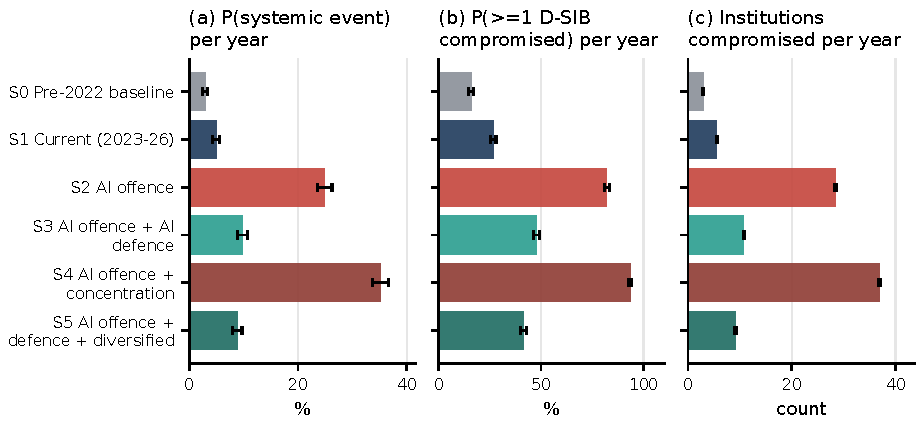
\includegraphics[width=\textwidth]{fig11_sim_scenarios.pdf}
\caption{Scenario outcomes with 95\% confidence intervals: (a) annual probability of a systemic event, (b) probability that at least one D-SIB is compromised, (c) institutions compromised per year.}
\label{fig:sim}
\end{figure}

Figure~\ref{fig:grid} varies the offence multiplier and the patch-time factor jointly. Offence dominates: at today's patch speed, the probability of a systemic event rises from 6\% to 45\% as the multiplier goes from 1 to 5. Faster patching alone has a modest effect. At a multiplier of 5, cutting patch times by 75\% lowers the probability only from 45\% to 40\%. When copycat exploitation starts within a day of disclosure and most damaging events begin as zero-days, the decisive defences act \emph{before} disclosure: pre-emptive discovery, smaller internet-facing exposure, detection and segmentation. This is the main operational lesson of the model.

\begin{figure}[!htbp]
\centering
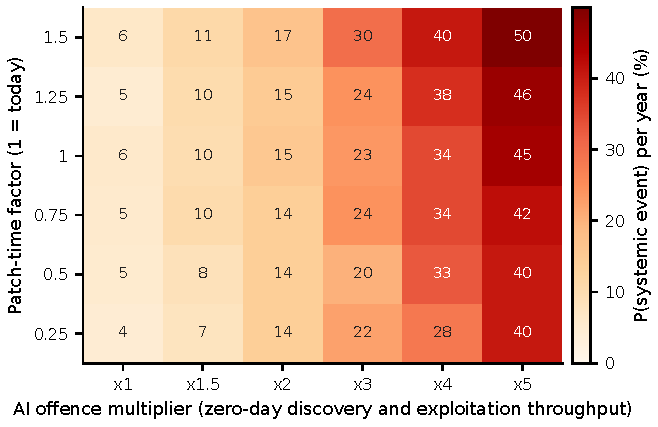
\includegraphics[width=0.78\textwidth]{fig12_sim_grid.pdf}
\caption{Annual probability of a systemic event (\%) by AI offence multiplier and patch-time factor (other parameters as in S2; 1,200 simulated years per cell).}
\label{fig:grid}
\end{figure}

\begin{table}[!htbp]
\centering
\caption{Robustness of scenario results to deployment probability $\rho$ and mass-campaign hit rate $c_{\text{mass}}$ (P(systemic) in \%, 1,000 years per cell).}
\label{tab:simrobust}
\scriptsize
\begin{tabular}{rrrrrrrrrrr}
\toprule
$\rho$ & $c_{\text{mass}}$ & S1 & S2 & S3 & S4 & S5 & S2/S1 & S3/S2 & S4/S2 & S5/S3 \\
\midrule
0.03 & 0.2 & 2.4 & 16.3 & 4.1 & 22.5 & 4.7 & 6.79 & 0.25 & 1.38 & 1.15 \\
0.03 & 0.3 & 4.0 & 16.0 & 6.6 & 26.3 & 4.4 & 4.00 & 0.41 & 1.64 & 0.67 \\
0.03 & 0.5 & 3.1 & 18.5 & 7.4 & 27.5 & 7.1 & 5.97 & 0.40 & 1.49 & 0.96 \\
0.05 & 0.2 & 4.1 & 25.9 & 8.2 & 36.0 & 7.9 & 6.32 & 0.32 & 1.39 & 0.96 \\
0.05 & 0.3 & 5.6 & 23.3 & 11.6 & 36.3 & 8.6 & 4.16 & 0.50 & 1.56 & 0.74 \\
0.05 & 0.5 & 5.8 & 27.0 & 11.0 & 40.1 & 10.9 & 4.66 & 0.41 & 1.49 & 0.99 \\
0.08 & 0.2 & 6.0 & 32.5 & 13.9 & 47.7 & 10.1 & 5.42 & 0.43 & 1.47 & 0.73 \\
0.08 & 0.3 & 8.4 & 36.2 & 13.8 & 49.2 & 11.7 & 4.31 & 0.38 & 1.36 & 0.85 \\
0.08 & 0.5 & 8.9 & 39.2 & 17.9 & 56.1 & 15.7 & 4.40 & 0.46 & 1.43 & 0.88 \\
\bottomrule
\end{tabular}
\end{table}

%=====================================================================
\section{Implications for central banks and the Bank of Thailand}\label{sec:policy}

\subsection{Should central banks pay attention?}
Yes, and the reason is specific to the evidence. Central banks meet this risk in three roles. As \emph{prudential supervisors}, they face a population of banks whose exposure is correlated through shared commercial products and providers, and whose patch workload has multiplied. As \emph{operators and overseers of payment infrastructure}, they run or supervise the nodes whose impairment turns an operational event into a systemic one \citep{cpmi2016guidance,eisenbach2022cyber}. As \emph{targets}, they hold sensitive supervisory and market data on the same commodity corporate IT that was compromised at the RBNZ and the EBA. AI changes each role: it multiplies discovery, shortens the effective response window, and gives defenders tools that are only effective if deployed sector-wide.

\paragraph{Is the BOT exposed?} The BOT's core settlement infrastructure scores low on vulnerability in our framework. Its corporate and supervisory IT, however, has a high target value and a moderate exposure profile (rank 9 of 12, risk 0.43), and it follows the pattern of the documented central-bank intrusions. The probability that the BOT experiences an intrusion through a commercial-product vulnerability over a multi-year horizon is not negligible. The probability that such an intrusion disrupts settlement is much lower, provided segmentation and contingency arrangements hold.

\subsection{Ten implications}
\begin{enumerate}[leftmargin=1.6em]
\item \textbf{Supervise patch latency on internet-facing products.} Treat time-to-remediate for known-exploited vulnerabilities in perimeter, MFT, mail and IT-management products as a prudential metric, with sector-wide reporting of patch-latency distributions and remediation targets measured in hours to days, not patch cycles.
\item \textbf{Build a shared-vendor concentration register.} Map which products and providers each institution uses in critical layers, compute concentration, and require substitution and isolation plans for dominant vendors. The model shows that concentration amplifies AI-driven risk by 36--64\%.
\item \textbf{Oversee critical third parties directly.} Shared IT and cloud providers rank highest in the Thai framework. Regimes for critical ICT third parties in other jurisdictions \citep{eu2022dora,boe2024ctp} offer templates for direct oversight, testing and incident obligations.
\item \textbf{Move defence before disclosure.} Because patch speed alone has diminishing returns, prioritise reducing internet-facing exposure, segmenting corporate IT from payment operations, detecting exploitation, and pre-emptive discovery in the software banks depend on.
\item \textbf{Pool AI-enabled defensive capacity.} Few Thai institutions can run frontier-model vulnerability research on their own. A sector capability---for example through TB-CERT with BOT support---could apply AI-assisted review to commonly used banking software, mobile-banking SDKs and cryptographic dependencies, and could coordinate access to restricted defensive programmes offered by AI developers \citep{anthropic2026glasswing}. Access to frontier models can itself be affected by foreign policy decisions: in June 2026 access to two frontier model families was temporarily suspended to comply with U.S.\ export controls and restored on 1 July \citep{anthropic2026access}. Contingency for such dependencies belongs in the plan.
\item \textbf{Prepare for the volume shock.} With advisories quadrupling, institutions must triage by exploitation evidence (KEV-type catalogues, exploitation prediction) rather than by severity scores alone \citep{jacobs2021epss}. A Thai or ASEAN exploited-vulnerability catalogue, mapped to products used locally, would help.
\item \textbf{Stress-test payment infrastructure for correlated impairment.} Scenario exercises should assume that several RTGS and retail-payment participants are impaired at once by a shared-product compromise, test offline and contingency settlement, and rehearse the kind of manual workaround used after the 2023 ICBC Financial Services incident.
\item \textbf{Harden the central bank's own corporate IT.} Apply the lessons of the RBNZ and EBA cases: minimise on-premise exposure of file-transfer and mail systems, enforce zero-trust access for supervisory data exchange, and keep settlement systems isolated from corporate networks.
\item \textbf{Govern AI platforms inside banks.} LLM gateways and workflow-automation tools became a KEV category in 2026. Banks should inventory them, treat internet-facing deployments as critical, and apply the same patch and access controls as for other perimeter software.
\item \textbf{Improve data and international coordination.} Adopt common incident-reporting formats \citep{fsb2023reporting,fsb2025fire}, collect Thai patch-latency and incident data to calibrate models like ours, and share threat intelligence through regional and BIS channels. Plan for hardware trust anchors as well: inventory HSM, secure-element and cryptographic-library dependencies and build crypto-agility into digital-asset, tokenisation and CBDC projects.
\end{enumerate}

\paragraph{Answer to RQ6.} Central banks should treat AI-accelerated vulnerability discovery as a financial-stability issue now. The aim is not to predict a specific attack. Under plausible parameters, the combination of a disclosure shock, correlated vendor exposure and AI-scaled offence raises systemic risk several-fold, and most of that increase can be offset only by coordinated, sector-wide defence.

%=====================================================================
\section{Limitations}\label{sec:limits}

\begin{itemize}
\item \textbf{Measurement of AI involvement.} Credits are incomplete (43\% coverage in 2026) and absent for the largest commercial CNAs. Tier~2 is a proxy. AI assistance at level L1 is invisible. We cannot attribute the disclosure surge to AI causally.
\item \textbf{KEV as ground truth.} KEV is curated by a U.S. agency, focuses on vulnerabilities relevant to U.S. federal systems, and lists exploitation when evidence becomes available. Listing lag is not the date exploitation began. Thai-specific exploitation may differ.
\item \textbf{Classification.} Product categories and software domains come from keyword rules. About 7\% of KEV entries and a larger share of AI-credited CVEs are unclassified.
\item \textbf{Curated cases and benchmarks.} The incident and hardware sets are purposive and author-coded from public reporting, and the industry zero-day counts used as benchmarks were taken from secondary reporting. All should be verified against primary sources.
\item \textbf{Thai framework.} The scores are structured judgements at group level, made without confidential supervisory data. They should be replaced with supervisory evidence where available.
\item \textbf{Simulation.} The model is stylised. Payment shares, patch speeds, success and disruption probabilities are assumptions, and only event rates are calibrated to data. Results are comparative across scenarios, not forecasts.
\item \textbf{Timing.} The data are a snapshot as of 12 November 2026. Rapid change in AI capability may make the trajectory estimates obsolete quickly.
\end{itemize}

%=====================================================================
\section{Conclusion}\label{sec:conclusion}

The economics of zero-days are changing. In 2026, vulnerability disclosure in major commercial software rose several-fold, AI systems were credited on more than a thousand CVEs, and the credited share doubled every few months. So far, exploitation has grown more slowly than discovery, which suggests that defenders are capturing much of the early benefit. The incident record shows that zero-days reach banks through the commercial products and service providers they share with everyone else. For a system such as Thailand's, the main systemic vulnerability is therefore correlated exposure through shared vendors and providers, not a bespoke attack on core payments. Our scenarios suggest that AI-scaled offence could multiply systemic risk several times over, and that coordinated AI-enabled defence, reduced exposure and attention to concentration can recover most of that loss. Central banks are positioned to organise that coordination, and the evidence argues for starting now.

\paragraph{Data and code availability.} All scripts, curated datasets, derived tables and figures are provided in the accompanying repository. Raw inputs are public: CVE List V5 (CVEProject/cvelistV5) and CISA KEV (cisagov/kev-data).

\paragraph{Acknowledgement of tools.} Data processing, analysis and drafting were assisted by an AI system; the author is responsible for the content.
